% Seminar slides: "Energy-Aware Agentic AI" -- Krish Tandel, IIT Bombay.
% Build: pdflatex slides.tex (twice). Fonts: Latin Modern (lmodern), as in the reference deck.
\documentclass[aspectratio=169,11pt,t]{beamer}
\usepackage[T1]{fontenc}
\usepackage{lmodern}
\usepackage{amsmath,amssymb,booktabs,graphicx,tikz,xcolor}
\usepackage[most]{tcolorbox}
\usetikzlibrary{arrows.meta,positioning,shapes.geometric,calc}

% ---------- colours sampled from the reference deck ----------
\definecolor{navy}{HTML}{0D2659}
\definecolor{rulegrey}{HTML}{9EA8BD}
\definecolor{secbg}{HTML}{F2F6F8}
\definecolor{defhead}{HTML}{1B5A7A}\definecolor{defbody}{HTML}{EBEBF7}
\definecolor{keyhead}{HTML}{EC5858}\definecolor{keybody}{HTML}{F7EBEB}
\definecolor{exhead}{HTML}{5EB2A8}\definecolor{exbody}{HTML}{EBF7EB}
\definecolor{footgrey}{HTML}{8C8C8C}
\definecolor{accent}{HTML}{EC5858}

% ---------- beamer look ----------
\setbeamertemplate{navigation symbols}{}
\setbeamercolor{normal text}{fg=black}
\setbeamercolor{structure}{fg=navy}
\setbeamerfont{frametitle}{family=\rmfamily,series=\bfseries,size=\Large}
\setbeamercolor{frametitle}{fg=navy}
\setbeamertemplate{frametitle}{%
  \vspace*{0.55em}\hspace*{0.1em}\insertframetitle\par\vspace{0.25em}%
  {\color{navy}\hrule height 0.6pt}\vspace{0.2em}}
\setbeamertemplate{itemize item}{\color{black}$\bullet$}
\setbeamertemplate{itemize subitem}{\scriptsize\raise0.2ex\hbox{\textendash}}
\setbeamertemplate{enumerate item}{\rmfamily\bfseries\color{navy}\insertenumlabel.}
\setbeamerfont{caption}{size=\footnotesize}
\setbeamertemplate{caption label separator}{: }
\setbeamercolor{caption name}{fg=navy}
\renewcommand{\figurename}{Figure}
\setbeamertemplate{footline}{%
  \leavevmode\hbox{\tiny\color{footgrey}%
  \hbox to 0.24\paperwidth{\hspace*{1.2em}\insertshortauthor\hfil}%
  \hbox to 0.47\paperwidth{\hfil\insertshorttitle\hfil}%
  \hbox to 0.29\paperwidth{\hfil\insertshortdate\hspace{1.2em}\insertframenumber/\inserttotalframenumber\hspace*{1.2em}}}%
  \vspace*{0.45em}}
\setbeamertemplate{title page}{%
  \vfill\centering
  {\usebeamerfont{title}\rmfamily\bfseries\color{navy}\inserttitle\par}\vspace{0.4em}
  {\rmfamily\large\color{navy}\insertsubtitle\par}\vspace{1.2em}
  {\rmfamily\insertauthor\par}\vspace{0.2em}
  {\rmfamily\footnotesize\insertinstitute\par}\vspace{1em}
  {\rmfamily\footnotesize\insertdate\par}\vfill}
\setbeamerfont{title}{size=\LARGE}
\setbeamertemplate{section page}{%
  \begin{tikzpicture}[remember picture,overlay]
    \fill[secbg] (current page.south west) rectangle (current page.north east);
  \end{tikzpicture}%
  \vfill\begin{minipage}{0.6\textwidth}
  {\sffamily\bfseries\large\insertsectionhead\par}\vspace{1.1em}
  {\color{rulegrey}\hrule height 0.5pt}\end{minipage}\vfill}
\AtBeginSection{{\setbeamertemplate{footline}{}\begin{frame}[plain,noframenumbering]\sectionpage\end{frame}}}

% ---------- blocks (as in the reference deck) ----------
\newtcolorbox{defbox}[1]{enhanced,colback=defbody,colframe=defhead,coltitle=white,boxrule=0pt,arc=1.5pt,
  left=4pt,right=4pt,top=2pt,bottom=3pt,toptitle=1pt,bottomtitle=1pt,fonttitle=\rmfamily\small,title={#1}}
\newtcolorbox{keybox}[1]{enhanced,colback=keybody,colframe=keyhead,coltitle=white,boxrule=0pt,arc=1.5pt,
  left=4pt,right=4pt,top=2pt,bottom=3pt,toptitle=1pt,bottomtitle=1pt,fonttitle=\rmfamily\small,title={#1}}
\newtcolorbox{exbox}[1]{enhanced,colback=exbody,colframe=exhead,coltitle=white,boxrule=0pt,arc=1.5pt,
  left=4pt,right=4pt,top=2pt,bottom=3pt,toptitle=1pt,bottomtitle=1pt,fonttitle=\rmfamily\small,title={#1}}
\newcommand{\hl}[1]{{\color{accent}\bfseries #1}}
\newcommand{\src}[1]{{\tiny\color{footgrey}#1}}

\title{Energy-Aware Agentic AI}
\subtitle{Iterative Repair, Its Energy Cost, and When to Stop}
\author{Krish Tandel}
\institute{Indian Institute of Technology Bombay}
\date{November 2026}

\begin{document}

{\setbeamertemplate{footline}{}\begin{frame}[noframenumbering]\titlepage\end{frame}}

\begin{frame}{Contents}
\rmfamily\bfseries\color{navy}
\begin{enumerate}\setlength{\itemsep}{0.9em}
\item Introduction
\item Foundations
\item Measuring Energy
\item Experiments on a Laptop GPU
\item Frontier-Scale Models
\item Conclusion
\end{enumerate}
\end{frame}

% =====================================================================
\section{Introduction}

\begin{frame}{One Prompt Is Cheap. An Agent Is Not.}
\begin{itemize}
\item<1-> One chatbot message: about \hl{0.6\,Wh}, less than a microwave uses in 10 seconds \src{[1]}
\item<2-> Data centres worldwide: \hl{485\,TWh} in 2025, projected \hl{950\,TWh} by 2030, about 3\% of global electricity \src{[2]}
\item<3-> An agent does not answer once: on SWE-bench, two top agents made \hl{28 and 51} model calls per task \src{[3]}
\end{itemize}
\vspace{0.6em}
\uncover<4->{%
\begin{defbox}{Agent}
A loop that \textbf{generates} an answer, \textbf{checks} it with a tool, and \textbf{decides} whether to try again. Every pass through the loop is another model call, and every call draws power.
\end{defbox}}
\end{frame}

\begin{frame}{The Question of This Seminar}
\centering
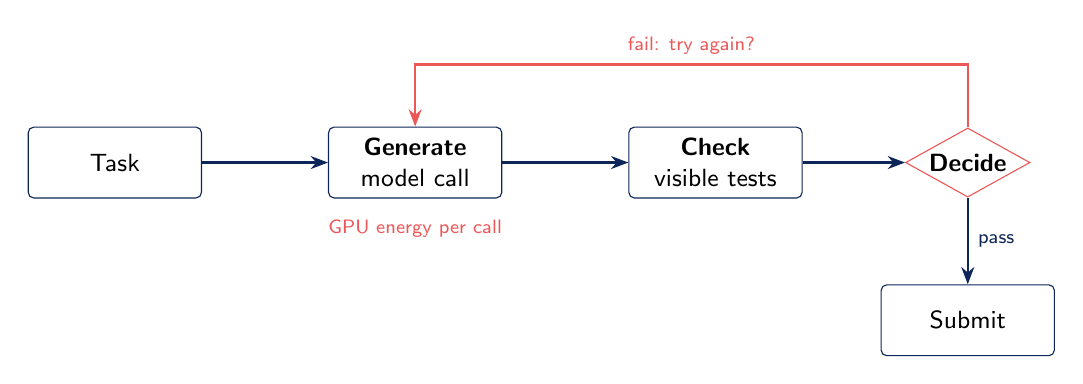
\begin{tikzpicture}[node distance=1.6cm, every node/.style={font=\sffamily\small},
  box/.style={draw=navy, rounded corners=2pt, minimum width=2.2cm, minimum height=0.9cm, align=center, fill=white},
  arr/.style={-{Stealth[length=2.2mm]}, thick, navy}]
\node[box] (t) {Task};
\node[box, right=of t] (g) {\textbf{Generate}\\model call};
\node[box, right=of g] (c) {\textbf{Check}\\visible tests};
\node[diamond, draw=accent, aspect=1.8, inner sep=1pt, right=1.3cm of c, font=\sffamily\small\bfseries] (d) {Decide};
\node[box, below=1.1cm of d] (s) {Submit};
\draw[arr] (t) -- (g); \draw[arr] (g) -- (c); \draw[arr] (c) -- (d);
\draw[arr] (d) -- node[right, font=\sffamily\scriptsize]{pass} (s);
\draw[arr, accent] (d.north) -- ++(0,0.8) -| node[pos=0.25, above, font=\sffamily\scriptsize, accent]{fail: try again?} (g.north);
\node[below=0.15cm of g, font=\sffamily\scriptsize, accent] {GPU energy per call};
\end{tikzpicture}
\vspace{0.3em}
\uncover<2->{%
\begin{keybox}{The question}
When the check fails, \textbf{is another AI step worth its energy?} If so, \textbf{how} should we spend it, and \textbf{when} should we stop?
\end{keybox}}
\end{frame}

% =====================================================================
\section{Foundations}

\begin{frame}{How a Language Model Produces an Answer}
\begin{itemize}
\item Text is split into \textbf{tokens}; the model predicts one token at a time
\item For each candidate token $i$ the network outputs a score $z_i$, and samples
\[ P(i) = \frac{e^{z_i/T}}{\sum_k e^{z_k/T}} \]
\item The \textbf{temperature} $T$ controls randomness (I used $T=0.2$)
\item<2-> Every token is a full pass through the network: \textbf{energy grows with tokens}, including hidden ``reasoning'' tokens the user never sees
\end{itemize}
\end{frame}

\begin{frame}{Ways to Spend an Extra Model Call}
\centering\footnotesize
\begin{tabular}{@{}p{2.7cm}p{3.2cm}p{3.3cm}p{3.3cm}@{}}
\toprule
\textbf{Strategy} & \textbf{Next call receives} & \textbf{Helps when} & \textbf{Main risk}\\
\midrule
Stop & nothing & first answers usually right & errors stay unfixed\\
\textbf{Fresh retry} & original task only & failures are random slips & repeats systematic errors\\
\textbf{Repair with feedback} & answer + failure message & feedback pinpoints the bug & anchors on its own answer\\
Self-correction & own critique, no tool & style fixes & no outside signal\\
Search or route & many candidates / bigger model & problem is too hard & cost multiplies\\
\bottomrule
\end{tabular}
\vspace{1em}
\begin{exbox}{Intuition: retrying with independent attempts}
If each attempt is right with probability $p$, then $\Pr(\text{at least one of } k) = 1-(1-p)^k$. For $p=0.5$, $k=2$: \textbf{75\%}. But attempts on a hard problem are \textbf{not} independent.
\end{exbox}
\end{frame}

\begin{frame}{A Running Example: The Collision Problem}
\begin{columns}[T]
\begin{column}{0.5\textwidth}
\small $n$ cars drive east, $n$ drive west; every eastbound car passes every westbound car once. \textbf{How many collisions?}
\vspace{0.6em}

\uncover<2->{\textbf{Model's first answer:}
\par\smallskip{\ttfamily\footnotesize def car\_race\_collision(n):\\\hspace*{2em}return {\color{accent}n}}\par\smallskip}
\uncover<3->{Visible test $n=1$: \textcolor{teal}{passes} (since $1 = 1^2$)\\}
\uncover<4->{Visible test $n=2$: \textcolor{accent}{fails}, expected 4}
\end{column}
\begin{column}{0.48\textwidth}
\uncover<5->{\textbf{After the failure message:}
\par\smallskip{\ttfamily\footnotesize def car\_race\_collision(n):\\\hspace*{2em}return {\color{teal}n * n}}\par\smallskip}
\uncover<6->{%
\begin{keybox}{But notice}
\small \texttt{return 4} also passes the $n=2$ test. Visible tests are an \textbf{incomplete verifier}, so I score every answer on EvalPlus's much larger \textbf{hidden} tests \src{[4]}.
\end{keybox}}
\end{column}
\end{columns}
\end{frame}

% =====================================================================
\section{Measuring Energy}

\begin{frame}{From GPU Power to Energy}
\begin{columns}[c]
\begin{column}{0.52\textwidth}
\begin{itemize}
\item \texttt{nvidia-smi} reads board power every \textbf{100\,ms}
\item Energy of request $r$ is the area under the curve:
\[ E_r \approx \sum_j \frac{P_j+P_{j+1}}{2}\,(t_{j+1}-t_j) \]
\item<2-> Collision run: \textbf{31.52\,J} (wrong) + \textbf{27.64\,J} (fix) = \hl{59.16\,J} for one correct answer
\end{itemize}
\end{column}
\begin{column}{0.46\textwidth}
\begin{figure}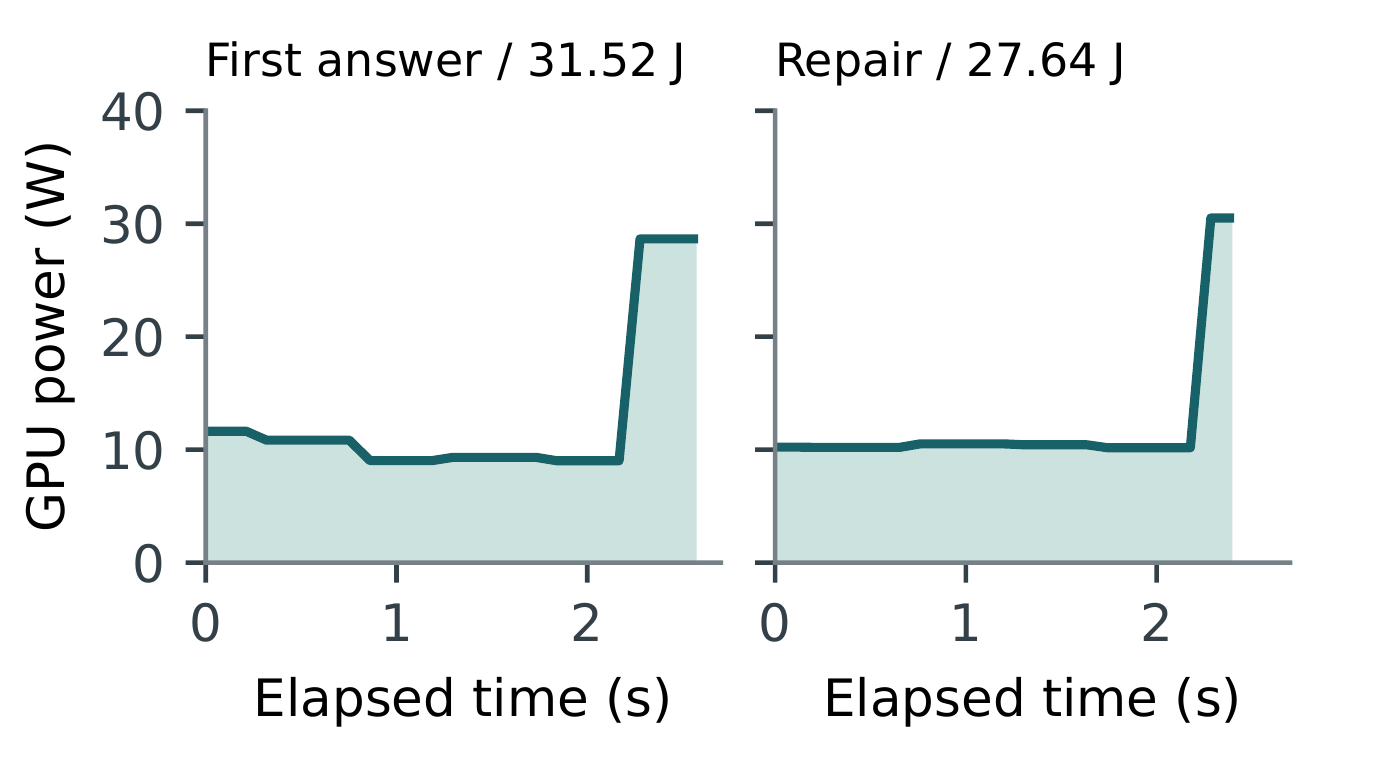
\includegraphics[width=\linewidth]{../report/figs/power_trace_original_crop.png}
\caption{Measured GPU power, collision run}\end{figure}
\end{column}
\end{columns}
\end{frame}

\begin{frame}{A Fair Metric: Energy per Correct Solution}
\[ J = \frac{\sum_i E_i}{\sum_i y_i} = \frac{\bar E}{\hat p} \qquad\text{(failed runs still cost energy)} \]
\uncover<2->{Policy $B$ beats policy $A$ only if
\[ J_B < J_A \iff \frac{\bar E_B}{\bar E_A} < \frac{\hat p_B}{\hat p_A} \]}
\uncover<3->{%
\begin{keybox}{Break-even rule}
If repair adds \textbf{10\% energy}, it must raise success by \textbf{more than 10\% (relative)} to be worth it.
\end{keybox}}
\uncover<4->{\small Emissions: $\times\,0.675$\,kg\,CO$_2$/kWh, India's grid average for FY 2025--26 \src{[5]}}
\end{frame}

% =====================================================================
\section{Experiments on a Laptop GPU}

\begin{frame}{Experimental Setup}
\begin{columns}[c]
\begin{column}{0.48\textwidth}
\begin{itemize}
\item RTX 5070 Laptop GPU, Ollama
\item Qwen2.5-Coder \textbf{1.5B} and \textbf{7B} (4-bit)
\item \textbf{Pilot:} 24 problems, 216 runs
\item \textbf{Follow-up:} 140 new problems, 383 runs, 1{,}128 measured requests
\item Hidden tests decide correctness; bootstrap 95\% intervals
\end{itemize}
\end{column}
\begin{column}{0.5\textwidth}
\centering
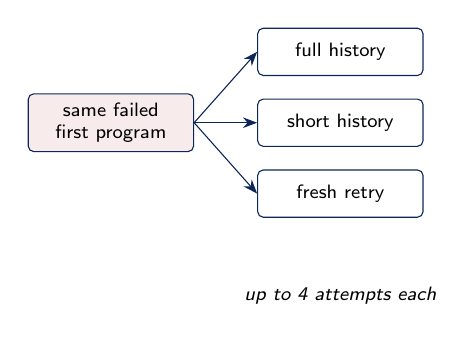
\begin{tikzpicture}[every node/.style={font=\sffamily\scriptsize},
  box/.style={draw=navy, rounded corners=2pt, minimum width=2.1cm, minimum height=0.6cm, align=center},
  arr/.style={-{Stealth[length=1.8mm]}, navy}]
\node[box, fill=keybody] (f) {same failed\\first program};
\node[box, right=0.8cm of f, yshift=0.9cm] (a) {full history};
\node[box, right=0.8cm of f] (b) {short history};
\node[box, right=0.8cm of f, yshift=-0.9cm] (c) {fresh retry};
\foreach \x in {a,b,c} \draw[arr] (f.east) -- (\x.west);
\node[below=0.75cm of c, align=center, font=\sffamily\scriptsize\itshape] {up to 4 attempts each};
\end{tikzpicture}
\vspace{0.4em}

\small Branching from \textbf{one} shared failure compares policies on identical cases.
\end{column}
\end{columns}
\end{frame}

\begin{frame}{Pilot: A Little Accuracy, A Lot of Energy}
\centering
\begin{tabular}{@{}lcccc@{}}
\toprule
Policy (Qwen 7B, 72 runs each) & Correct & Success & J/run & \textbf{J/correct}\\
\midrule
One attempt & 60/72 & 83.3\% & 107.1 & \textbf{128.5}\\
Full history & 62/72 & 86.1\% & 163.0 & 189.3\\
Short history & 63/72 & 87.5\% & 154.4 & 176.4\\
\bottomrule
\end{tabular}
\vspace{1em}
\begin{itemize}
\item<2-> Energy per run \textbf{+44--52\%}; success only \textbf{+3--5\%} (relative)
\item<3-> All 13 runs that hit the 4-attempt cap still failed, yet used \textbf{38--44\%} of the energy
\end{itemize}
\end{frame}

\begin{frame}{Surprise \#1: The Model Repeats Itself}
\begin{columns}[c]
\begin{column}{0.58\textwidth}
\uncover<2->{\begin{figure}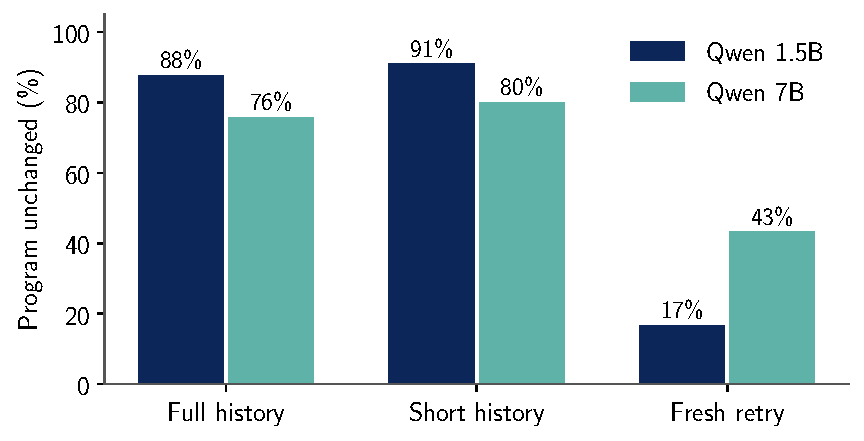
\includegraphics[width=\linewidth]{figs/unchanged.pdf}
\caption{Share of continuation attempts that returned the same program again}\end{figure}}
\end{column}
\begin{column}{0.4\textwidth}
\small Shown its own failure message, how often does the model change its code?
\vspace{0.6em}

\uncover<3->{It resubmitted the \textbf{identical program} in \hl{76--91\%} of repair attempts.}
\vspace{0.6em}

\uncover<4->{Short or full history? \textbf{No measurable difference} (energy ratio 0.98--1.01).}
\end{column}
\end{columns}
\end{frame}

\begin{frame}{New Experiment: Is It Just the Low Temperature?}
\begin{columns}[c]
\begin{column}{0.58\textwidth}
\uncover<2->{\begin{figure}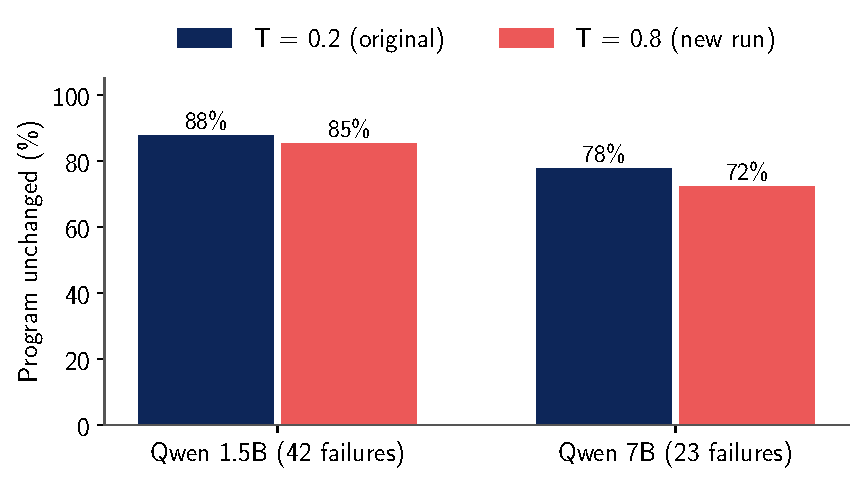
\includegraphics[width=0.92\linewidth]{figs/temperature.pdf}
\caption{Full-history repair rerun at $T=0.8$ from the same failed programs (seed 11)}\end{figure}}
\end{column}
\begin{column}{0.4\textwidth}
\footnotesize
\begin{itemize}\setlength{\itemsep}{0.2em}
\item Objection: at $T=0.2$ the model is too deterministic to change its code
\item Test: rerun every repair at $T=0.8$ from the same failed answers
\item<2-> Still \hl{85\%} (1.5B) and \hl{72\%} (7B) unchanged
\item<3-> Correct after repair (hidden tests): 2 $\to$ 2 (1.5B), 1 $\to$ 2 (7B)
\end{itemize}
\uncover<4->{\begin{keybox}{Insight}Not randomness: the model is \textbf{confident in its wrong answer}.\end{keybox}}
\end{column}
\end{columns}
\end{frame}

\begin{frame}{Live Demo: Repair vs.\ Fresh Retry}
\small Same problem (HumanEval/134), Qwen 1.5B, laptop GPU:\\ \texttt{python live\_demo.py -{}-task HumanEval/134}
\vspace{0.6em}
\begin{columns}[T]
\begin{column}{0.48\textwidth}
\begin{defbox}{Repair with feedback}
\begin{tabular}{@{}lll@{}}
Attempt & Visible tests & Energy\\
\midrule
1 & 9/10 \textcolor{accent}{fail} & 84.5\,J\\
2 & 9/10 \textcolor{accent}{fail} & 96.4\,J\\
3 & 9/10 \textcolor{accent}{fail} & 100.3\,J\\
4 & 9/10 \textcolor{accent}{fail} & 90.9\,J\\
\midrule
\multicolumn{2}{@{}l}{\textbf{Same program 4 times}} & \textbf{372\,J}
\end{tabular}
\end{defbox}
\end{column}
\begin{column}{0.48\textwidth}
\uncover<2->{%
\begin{exbox}{Fresh retry}
\begin{tabular}{@{}lll@{}}
Attempt & Visible tests & Energy\\
\midrule
1 & 9/10 \textcolor{accent}{fail} & 77.0\,J\\
2 & 10/10 \textcolor{teal}{pass} & 96.4\,J\\
\midrule
\multicolumn{2}{@{}l}{\textbf{Solved in 2 attempts}} & \textbf{173\,J}
\end{tabular}
\end{exbox}}
\end{column}
\end{columns}
\vspace{0.4em}
\uncover<3->{\src{Rehearsal run, 21 November 2026. Energy varies run to run; the pattern is the point.}}
\end{frame}


\begin{frame}{Surprise \#2: Starting Over Beats Fixing}
\begin{columns}[c]
\begin{column}{0.58\textwidth}
\begin{figure}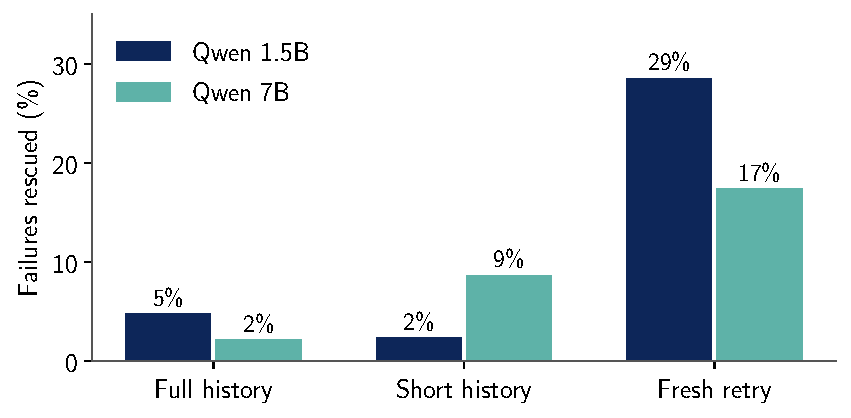
\includegraphics[width=\linewidth]{figs/rescues.pdf}
\caption{Failed first answers turned into correct ones (cap 4)}\end{figure}
\end{column}
\begin{column}{0.4\textwidth}
\small
\begin{itemize}
\item A fresh retry rescued \textbf{12 of 42} (1.5B) and \textbf{8 of 46} (7B) failures
\item Repair rescued \textbf{at most 4}
\item<2-> Yet \textbf{no} multi-attempt policy beat one attempt on energy per correct solution
\end{itemize}
\uncover<3->{\begin{keybox}{Lesson}Retrying buys accuracy, not efficiency.\end{keybox}}
\end{column}
\end{columns}
\end{frame}

\begin{frame}{When to Stop? A ``No Progress'' Rule}
\begin{defbox}{Progress-based stop (patience $K$)}
Count visible checks passed at each attempt; stop when there has been no improvement for $K$ attempts.
\end{defbox}
\vspace{0.4em}
\begin{itemize}
\item<2-> For repair, $K=1$ kept almost every rescue at \textbf{a quarter to a third less energy} than a 4-attempt cap
\item<3-> \ldots but because repair repeats itself, it almost always stopped at attempt 2: \textbf{a plain cap of 2 does the same}
\item<4-> For fresh retries it is the \textbf{wrong signal}: it threw away 5 of 12 (1.5B) rescues
\end{itemize}
\uncover<5->{\begin{keybox}{Takeaway}A fixed attempt budget is simpler and safer.\end{keybox}}
\end{frame}

\begin{frame}{Small Model + Retries vs.\ Large Model Once}
\begin{columns}[c]
\begin{column}{0.58\textwidth}
\begin{figure}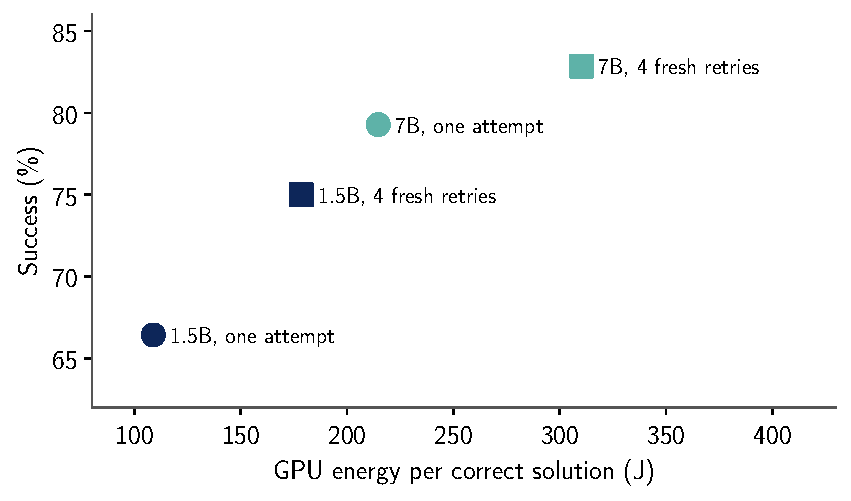
\includegraphics[width=\linewidth]{figs/tradeoff.pdf}
\caption{Same 140 problems, seed 11}\end{figure}
\end{column}
\begin{column}{0.4\textwidth}
\small
\begin{itemize}
\item 7B, one attempt: \textbf{79.3\%}
\item<2-> 1.5B + 4 fresh retries: \textbf{75.0\%}
\item<3-> \ldots at \hl{0.83$\times$} the energy per correct solution
\end{itemize}
\uncover<4->{Neither gap is statistically clear: a small model that retries is a \textbf{serious alternative}, not a proven winner.}
\end{column}
\end{columns}
\end{frame}

% =====================================================================
\section{Frontier-Scale Models}

\begin{frame}{Scaling Up to 2.8 Trillion Parameters}
\begin{columns}[c]
\begin{column}{0.6\textwidth}
\only<1>{\begin{figure}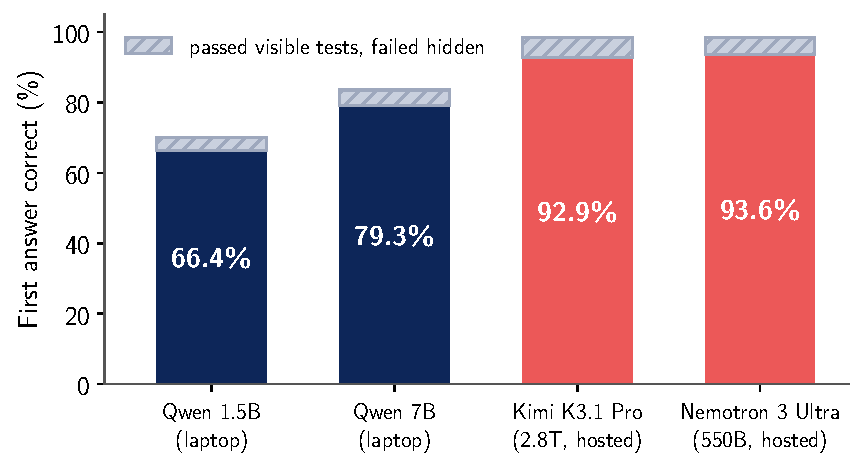
\includegraphics[width=\linewidth]{figs/fourmodels.pdf}\caption{First attempt; hosted runs via OpenRouter}\end{figure}}
\only<2->{\begin{figure}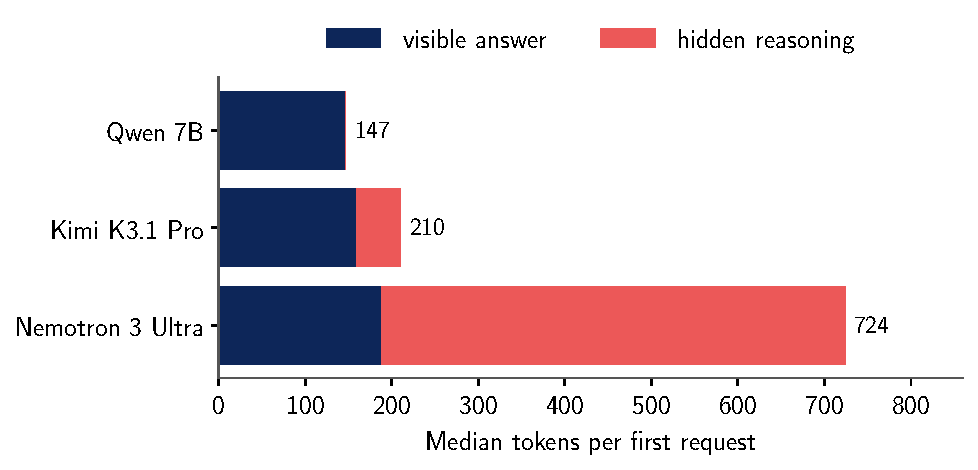
\includegraphics[width=\linewidth]{figs/tokens.pdf}\caption{Hidden reasoning before each answer}\end{figure}}
\end{column}
\begin{column}{0.38\textwidth}
\small
\begin{itemize}
\item Kimi K3.1 Pro (2.8T) \textbf{92.9\%}, Nemotron 3 Ultra (550B) \textbf{93.6\%}: \textbf{+14 points} over 7B
\item Scale beats retries: 1.5B + retries is still \textbf{18 points} behind
\item<2-> Nemotron thinks \textbf{536} tokens (median) before answering; on average reasoning is \textbf{6$\times$} the visible answer
\item<2-> Kimi's whole run cost \textbf{\$0.46}
\end{itemize}
\end{column}
\end{columns}
\end{frame}

\begin{frame}{Surprise \#3: Bigger Models Still Fool the Checker}
\begin{itemize}
\item 7--8 first answers per large model \textbf{passed every visible test} but failed the hidden ones
\item That is \textbf{more} than either small model (5--6)
\item<2-> No stopping rule can catch these: only a \textbf{better verifier} can
\end{itemize}
\vspace{0.6em}
\uncover<3->{%
\begin{defbox}{Energy you cannot see}
Google measures a median Gemini text prompt at \textbf{0.24\,Wh} (0.10\,Wh for accelerators alone, $\approx$360\,J) \src{[6]}. My laptop's median first request: \textbf{152\,J} (7B). Same order of magnitude, but a request with a thousand reasoning tokens sits well above the median, and API users see tokens and prices, \textbf{never energy}.
\end{defbox}}
\end{frame}

% =====================================================================
\section{Conclusion}

\begin{frame}{Policy: Tell Users Why the Agent Stopped}
\begin{itemize}
\item India's AI Governance Guidelines ask for \emph{Accountability} and \emph{Understandable by Design} \src{[7]}
\item They prescribe no energy logs; applying the principles, every agent answer could carry a short record:
\end{itemize}
\vspace{0.6em}
\centering
\begin{tabular}{@{}ll@{}}
\toprule
Field & Collision run (HumanEval/41)\\
\midrule
Stopping reason & visible test passed (attempt 2 of 4)\\
Energy and boundary & 59.16\,J, GPU board, inference only\\
Tokens (incl.\ hidden reasoning) & logged per request\\
\bottomrule
\end{tabular}
\end{frame}

\begin{frame}{Summary and Future Directions}
\begin{keybox}{Summary}
\begin{itemize}\small
\item One attempt gives the \textbf{lowest energy per correct solution}
\item Repair mostly \textbf{repeats the same program}; a \textbf{fresh retry} rescues far more failures
\item A ``no progress'' stop equals a \textbf{cap of two}; use a fixed budget
\item Frontier models: \textbf{93\%} first time, but hidden reasoning multiplies cost and wrong answers still pass weak checks
\end{itemize}
\end{keybox}
\begin{defbox}{Not answered}
\small Energy of hosted models (only operators can measure it); repository-scale agents; whole-system energy beyond the GPU board.
\end{defbox}
\end{frame}

\begin{frame}{References}
\footnotesize
\begin{itemize}\setlength{\itemsep}{0.25em}
\item[{[1]}] Epoch AI (2026), ``What you need to know about AI energy use'', epoch.ai/publications/ai-energy
\item[{[2]}] IEA (2026), \emph{Key Questions on Energy and AI}, iea.org (CC BY 4.0)
\item[{[3]}] SWE-bench experiments repository, SWE-bench Verified submissions (GPT-5.2 Codex, Gemini 3 Pro), github.com/SWE-bench/experiments
\item[{[4]}] J.\ Liu et al., ``Is Your Code Generated by ChatGPT Really Correct?'', NeurIPS 2023 (EvalPlus)
\item[{[5]}] Central Electricity Authority, CO$_2$ Baseline Database v22.0, 2026
\item[{[6]}] C.\ Elsworth et al., ``Measuring the environmental impact of delivering AI at Google scale'', arXiv:2508.15734
\item[{[7]}] MeitY, \emph{India AI Governance Guidelines}, November 2025
\item[{[8]}] Code and data: github.com/2kri5h/Seminar-Autumn-26
\end{itemize}
\end{frame}

\end{document}
